% !TEX program = xelatex
\documentclass[UTF8,11pt,scheme=chinese,fontset=fandol]{ctexart}

\usepackage[a4paper,margin=2.25cm]{geometry}
\usepackage{amsmath,amssymb,amsthm,mathtools}
\usepackage{booktabs,longtable,tabularx,array}
\usepackage{graphicx,float}
\usepackage{xcolor}
\usepackage{enumitem}
\usepackage[hidelinks]{hyperref}

\graphicspath{{../../figures/}}
\setlength{\parindent}{2em}
\setlength{\parskip}{0.25em}
\renewcommand{\arraystretch}{1.25}
\setlist[itemize]{leftmargin=2.2em,itemsep=0.25em,topsep=0.35em}
\setlist[enumerate]{leftmargin=2.4em,itemsep=0.25em,topsep=0.35em}
\setcounter{tocdepth}{2}

\definecolor{deepblue}{RGB}{0,72,122}
\definecolor{darkgreen}{RGB}{0,110,75}
\definecolor{warmred}{RGB}{165,55,45}

\newcommand{\calB}{\mathcal B}
\newcommand{\calD}{\mathcal D}
\newcommand{\calP}{\mathcal P}
\newcommand{\MG}{\mathcal M_G}

\theoremstyle{definition}
\newtheorem{learninggoal}{学习目标}[section]
\newtheorem{intuition}{经济直觉}[section]
\newtheorem{workedexample}{例题}[section]
\newtheorem{commonerror}{易错点}[section]
\newtheorem{optionalmath}{选读推导}[section]

\title{\textbf{统一市场、数字平台与地方收入}\\[0.45em]
\large 本科生讲义：一般需求系统与当前 M1--M3 版本}
\author{依据 Wenxiao Dong 与 Yaqi Hu 的理论短文整理\\
\small 独立教学版本，不替代旧讲义或投稿论文}
\date{2026 年 7 月}

\begin{document}

\maketitle

\begin{abstract}
这份讲义面向学过中级微观经济学和基础微积分的本科生。它研究一个看似简单、但容易被
“交易额”掩盖的问题：平台让商品更便宜、市场更大以后，消费发生地是否也能保留相应的
收入？讲义从一笔 100 元平台订单出发，逐步建立家庭需求、渠道留值和地方收入循环，随后
解释当前论文的三个核心结果：有限整合冲击存在两个能力阈值（M1），边际价值捕获拖累在
一般需求系统下仍然单峰（M2），市场整合与地方组织能力在对数收入上具有 increasing
differences（M3）。CES 只作为一个可计算特例。全文包含数值例子、图形阅读、分层练习和
参考答案，不要求学生掌握一般均衡或高级动态优化。
\end{abstract}

\noindent\textbf{版本说明。}本文件是新建的本科生版本。旧讲义
\texttt{EL\_model\_teaching\_note\_zh.tex} 及其 PDF 保持不变；旧讲义记录了论文较早的
CES／局部阈值版本，本讲义则与当前一般需求系统及有限变化结果一致。

\tableofcontents
\clearpage

\section{从一笔 100 元平台订单开始}

居民在本地用手机下单 100 元，并不表示这 100 元都会成为本地收入。订单至少可以被拆成
以下几部分：生产者收入、平台服务费、仓储与履约收入、运输收入、本地销售和售后服务
收入。只有其中支付给本地劳动、本地服务和本地所有者的部分，才会进入本地收入账户。

因此要区分两个地点：
\begin{itemize}
  \item \textbf{消费发生地}：居民在哪里付款和收货；
  \item \textbf{收入形成地}：工资、利润和服务收入最终归属于哪里。
\end{itemize}

平台可能同时带来三条作用链：
\[
\boxed{
\begin{aligned}
\text{整合 }z\uparrow
&\Longrightarrow \text{外部市场更容易进入}
&&\Longrightarrow \text{基础收入 }B\text{ 可能增加},\\
z\uparrow
&\Longrightarrow p_P\downarrow
&&\Longrightarrow \text{消费价格指数 }P_M\downarrow,\\
z\uparrow
&\Longrightarrow \text{平台支出份额 }s\uparrow
&&\Longrightarrow \text{本地平均留值率 }\omega\text{ 改变}.
\end{aligned}}
\]

前两条通常是 access gain 和 consumer-price gain；第三条是 local value capture。三者共同
决定本地名义收入和消费购买力，不能只看平台交易额。

\begin{learninggoal}
完成本讲义后，学生应能：（1）区分支出与本地收入；（2）解释平台支出份额为何等于价格
指数的弹性；（3）从收入固定点得到两种地方乘数；（4）用能力阈值判断有限整合冲击的三个
结果区域；（5）解释 capture drag 为什么单峰；（6）准确说明 M3 的含义和边界。
\end{learninggoal}

\section{模型地图：对象、顺序与边界}

模型研究一个无法影响外部价格和工资的 small open region。外部商品价格和本地工资都
规范化为 1。整合指数 \(z\in\mathbb R\) 降低平台渠道价格：
\[
p_P(z)=\bar p_Pe^{-z},
\qquad \frac{d\ln p_P}{dz}=-1.
\]
本地自主收入写为
\[
B(z)=\bar Be^{\varepsilon z},
\qquad \frac{d\ln B}{dz}=\varepsilon\geq0.
\]
沿研究路径假定两渠道的 Hicksian demands 唯一且内部，并且
\[
s(z)\in(0,1),\qquad s'(z)>0.
\]

模型按以下顺序闭合：
\[
\boxed{
(z,p_A,p_P)\ \longrightarrow\ (P_M,s)\ \longrightarrow\
(\rho_P,\Delta,\omega)\ \longrightarrow\ (D,Y,R).}
\]
组织能力 \(\kappa\) 只进入平台留值率，不改变价格、偏好或需求份额路径。

\begin{center}
\small
\begin{tabularx}{\textwidth}{>{\centering\arraybackslash}p{1.8cm}p{3.4cm}X}
\toprule
符号 & 名称 & 经济含义 \\
\midrule
\(z\) & 市场整合指数 & 越大表示平台渠道相对价格越低、平台渗透越深 \\
\(s\) & 平台支出份额 & 零售支出中通过平台渠道完成的比例，不是数量份额 \\
\(\kappa\) & 地方组织能力 & 本地卖家参与、履约、配套服务和组织协调的外生概括 \\
\(\rho_A,\rho_P\) & 渠道留值率 & 一元渠道交易中成为本地要素和所有者收入的比例 \\
\(\omega\) & 平均留值率 & 按渠道支出份额加权后的本地价值捕获比例 \\
\(B\) & 自主本地收入 & 进入模型时已经是本地收入，例如外销增加值 \\
\(G\) & 外部融资零售支出 & 进入模型时仍是总支出，例如游客在本地消费 \\
\(Y\) & 名义本地收入 & 所有收入传播轮次完成后的均衡收入 \\
\(R\) & 消费等价实际收入 & 在模型消费篮子中的购买力，不是完整社会福利 \\
\bottomrule
\end{tabularx}
\end{center}
\normalsize

\begin{commonerror}
不要把 \(z\)、\(s\) 和 \(\kappa\) 当作同一个变量。\(z\) 是外生整合冲击，\(s\) 是家庭
需求产生的平台支出份额，\(\kappa\) 是改变平台交易本地留值率的能力参数。
\end{commonerror}

\section{家庭需求：先做外层，再理解渠道内层}

\subsection{外层支出分配}

居民消费零售综合品 \(M\)、本地非贸易品 \(N\) 和外部商品 \(Z\)：
\[
\max_{M,N,Z\geq0}M^\alpha N^\beta Z^{1-\alpha-\beta}
\quad\text{s.t.}\quad P_MM+N+Z=Y,
\]
其中 \(\alpha,\beta>0\) 且 \(\alpha+\beta<1\)。Cobb--Douglas 的一阶条件给出固定支出
份额：
\[
P_MM=\alpha Y,
\qquad N=\beta Y,
\qquad Z=(1-\alpha-\beta)Y.
\]
把最优消费代回效用，可得到消费等价实际收入
\[
R=K\frac{Y}{P_M^\alpha},
\qquad
K=\alpha^\alpha\beta^\beta
(1-\alpha-\beta)^{1-\alpha-\beta}.
\]

所以 \(Y\) 衡量“赚了多少名义收入”，\(R\) 同时考虑名义收入和零售价格指数。若平台使
\(P_M\) 下降，即使 \(Y\) 略降，\(R\) 仍可能上升。

\subsection{一般两渠道需求}

零售综合品 \(M\) 可以通过本地代理渠道 \(A\) 或外部平台渠道 \(P\) 获得。主模型不要求
CES，只要求两渠道聚合器严格递增、线性齐次，并有可微的单位支出函数
\(P_M(p_A,p_P)\)。

令 \(h_P(p_A,p_P,1)\) 是获得一单位 \(M\) 时的平台 Hicksian demand。Shephard's lemma
给出
\[
\frac{\partial P_M}{\partial p_P}=h_P(p_A,p_P,1).
\]
因此平台支出份额为
\[
s
=\frac{p_Ph_P}{P_M}
=\frac{\partial\ln P_M}{\partial\ln p_P}
\in(0,1).
\]
沿整合路径 \(d\ln p_P/dz=-1\)，链式法则立即得到
\[
\boxed{\frac{d\ln P_M}{dz}=-s.}
\]

\begin{intuition}
若平台支出份额为 0.3，平台价格按比例下降 1\%，零售价格指数在局部近似下降 0.3\%。
这个结论来自支出最小化和包络性质，不依赖 CES 闭式解。
\end{intuition}

\section{地方留值：平台交易中有多少成为本地收入}

本地代理渠道的留值率为 \(\rho_A\in[0,1]\)。平台留值率随地方组织能力增加：
\[
\rho_P(\kappa)=\underline\rho_P+\kappa\delta_\rho,
\qquad
\delta_\rho=\overline\rho_P-\underline\rho_P>0,
\qquad \kappa\in[0,1].
\]
并假定
\[
0\leq\underline\rho_P<\overline\rho_P\leq1.
\]
这里的 \(\kappa\) 可以理解为本地卖家的数字化参与、仓储履约、售后服务、合作组织与议价
协调等能力的综合指标。模型把它视为外生 retention shifter，不求解最优能力投资。

定义渠道留值差
\[
\Delta(\kappa)=\rho_A-\rho_P(\kappa).
\]
按平台支出份额加权，平均本地留值率为
\begin{align*}
\omega(z,\kappa)
&=(1-s)\rho_A+s\rho_P(\kappa)\\
&=\rho_A-s\Delta(\kappa).
\end{align*}
两个导数揭示了全部方向：
\[
\omega_z=-\Delta(\kappa)s'(z),
\qquad
\omega_\kappa=s\delta_\rho>0.
\]

\begin{center}
\begin{tabular}{ccl}
\toprule
条件 & 平台扩张对 \(\omega\) 的影响 & 解释 \\
\midrule
\(\Delta>0\) & \(\omega_z<0\) & 平台留值低于本地代理，出现 capture leakage \\
\(\Delta=0\) & \(\omega_z=0\) & 渠道重组不改变本地平均留值率 \\
\(\Delta<0\) & \(\omega_z>0\) & 平台留值更高，平台扩张提高本地捕获 \\
\bottomrule
\end{tabular}
\end{center}

\begin{commonerror}
\(\rho_P\)、\(\omega\) 和 \(\Delta\) 不是同一个对象。\(\rho_P\) 是平台渠道自身的
留值率，\(\omega\) 是全体零售支出的平均留值率，\(\Delta\) 是两个渠道留值率之差。
\end{commonerror}

\section{地方收入固定点与两种 benchmark multipliers}

\subsection{为什么收入会循环}

本地收入一部分用于本地非贸易品，一部分用于零售综合品；这些支出又形成新的本地工资和
企业收入。均衡收入满足
\[
\boxed{Y=B+\beta Y+\omega(\alpha Y+G).}
\]
右侧四项分别是：
\begin{itemize}
  \item 已经成为本地收入的自主注入 \(B\)；
  \item 本地非贸易品支出形成的收入 \(\beta Y\)；
  \item 居民零售支出中留在本地的部分 \(\omega\alpha Y\)；
  \item 外部融资零售支出中留在本地的部分 \(\omega G\)。
\end{itemize}

整理得到
\[
Y=\frac{B+\omega G}{D},
\qquad
D=1-\beta-\alpha\omega
=d_A+\alpha s\Delta(\kappa),
\qquad
d_A=1-\beta-\alpha\rho_A>0.
\]
因为 \(0\leq\omega\leq1\) 且 \(\alpha+\beta<1\)，传播系数
\(\beta+\alpha\omega<1\)，所以固定点唯一，几何级数收敛。

\subsection{为什么有两种乘数}

对 \(B\) 和 \(G\) 分别求导：
\[
\boxed{
m_B=\frac{\partial Y}{\partial B}=\frac1D,
\qquad
\MG=\frac{\partial Y}{\partial G}=\frac{\omega}{D}.}
\]

\begin{workedexample}[100 元注入]
取 \(\alpha=0.35\)、\(\beta=0.25\)、\(s=0.25\)、\(\rho_A=0.8\)、
\(\rho_P=0.35\)。此时
\[
\omega=0.75(0.8)+0.25(0.35)=0.6875,
\qquad D=0.509375.
\]
若 100 元在进入模型时已经是本地收入，最终收入增加
\[
100m_B=100/0.509375=196.319.
\]
若 100 元只是游客等外部主体支付的零售支出，第一轮只有
\(100\omega=68.75\) 元成为本地收入，最终增加
\[
100\MG=100(0.6875)/0.509375=134.969.
\]
两者的差异发生在第一轮；之后都按 \(\beta+\alpha\omega=0.490625\) 继续传播。
\end{workedexample}

\begin{commonerror}
\(B\) 与 \(G\) 不能互换。外销增加值可以进入 \(B\)，因为它已经是本地收入；游客的一元
消费进入 \(G\)，因为其中只有 \(\omega\) 成为第一轮本地收入。
\end{commonerror}

\section{M1：有限整合冲击与两个能力阈值}

M1 研究从 \(z_0\) 到 \(z_1>z_0\) 的有限变化，而不是只看某一点的导数。为获得透明的
闭式阈值，本节设 \(G=0\)。记
\[
s_j=s(z_j),\quad B_j=B(z_j),\quad P_{Mj}=P_M(z_j),
\]
并定义
\[
D_j(\kappa)=d_A+\alpha s_j\Delta(\kappa),
\quad
\calB=\frac{B_1}{B_0},
\quad
\calP=\frac{P_{M1}}{P_{M0}},
\quad
\calD(\kappa)=\frac{D_1(\kappa)}{D_0(\kappa)}.
\]
因为整合使平台价格下降和平台支出份额上升，\(0<\calP<1\) 且 \(s_1>s_0\)。两种收入
的有限变化为
\[
\boxed{
\frac{Y_1}{Y_0}=\frac{\calB}{\calD(\kappa)},
\qquad
\frac{R_1}{R_0}=\frac{\calB}
{\calD(\kappa)\calP^\alpha}.}
\]
组织能力不改变 \(B_j\)、\(s_j\) 或 \(P_{Mj}\)，只削弱捕获分母的恶化：
\[
\frac{\partial\ln\calD}{\partial\kappa}
=-\frac{\alpha\delta_\rho d_A(s_1-s_0)}{D_1D_0}<0.
\]

定义两个“需要被跨越的目标”：
\[
q_Y^F=\calB,
\qquad
q_R^F=\frac{\calB}{\calP^\alpha}.
\]
由于 \(0<\calP<1\)，所以 \(q_R^F>q_Y^F\)。若满足 endpoint-crossing 条件
\[
\boxed{\calD(0)>q_R^F>q_Y^F>\calD(1),}
\]
则存在唯一内部阈值
\[
0<\kappa_R^F<\kappa_Y^F<1.
\]
对上述可达区间 \(q\in(\calD(1),\calD(0))\) 内的任一目标，阈值可写为
\[
\kappa(q)=\frac1{\delta_\rho}
\left[\Delta_0-
\frac{(q-1)d_A}{\alpha(s_1-qs_0)}\right],
\qquad
\Delta_0=\rho_A-\underline\rho_P.
\]

\begin{center}
\small
\begin{tabular}{cll}
\toprule
能力区域 & 名义本地收入 \(Y\) & 消费等价实际收入 \(R\) \\
\midrule
\(0\leq\kappa<\kappa_R^F\) & 下降 & 下降 \\
\(\kappa_R^F<\kappa<\kappa_Y^F\) & 下降 & 上升 \\
\(\kappa_Y^F<\kappa\leq1\) & 上升 & 上升 \\
\bottomrule
\end{tabular}
\end{center}

在 \(\kappa_R^F\) 处，\(R_1/R_0=1\) 但 \(Y_1/Y_0=\calP^\alpha<1\)；在
\(\kappa_Y^F\) 处，\(Y_1/Y_0=1\) 但 \(R_1/R_0=\calP^{-\alpha}>1\)。实际收入较早
转正，是因为它还得到价格指数下降的收益。

\begin{workedexample}[当前图形参数]
采用
\[
\alpha=.35,\ \beta=.25,\ a=.4,\ \eta=4,\ \varepsilon=.08,
\quad p_A=\bar p_P=1,
\quad \rho_A=.8,
\quad (\underline\rho_P,\overline\rho_P)=(.1,.6),
\]
以及 \((z_0,z_1)=(-.75,-.30)\)。CES 在这里只用于生成一个可计算的 share path。数值为
\[
s_0=.065653,\quad s_1=.213247,\quad
\calP=.944300,\quad \calB=1.036656,
\]
\[
q_R^F=1.057660,\qquad q_Y^F=1.036656,
\qquad
\boxed{\kappa_R^F=.323162<\kappa_Y^F=.721929.}
\]

\begin{center}
\begin{tabular}{cccl}
\toprule
\(\kappa\) & \(Y_1/Y_0\) & \(R_1/R_0\) & 结果 \\
\midrule
0 & .964877 & .984427 & 两者都下降 \\
.5 & .988803 & 1.008837 & 名义收入下降，实际收入上升 \\
1 & 1.014569 & 1.035126 & 两者都上升 \\
\bottomrule
\end{tabular}
\end{center}
这些参数只用于机制说明，不是 calibration。
\end{workedexample}

\begin{commonerror}
只有目标位于 \((\calD(1),\calD(0))\) 内时，才存在内部阈值。目标等于端点时阈值位于
0 或 1；目标在闭区间外时没有 crossing。不能在任何参数下机械报告两个阈值。
\end{commonerror}

\section{M2：capture drag 为什么仍然只有一个峰}

\subsection{从 share-speed 到边际收入分解}

把平台份额对整合的反应写成
\[
s'(z)=g(s).
\]
\(g(s)\) 是 share-speed：它衡量整合提高一点时，支出向平台重配得有多快。设
\(G=0\) 并在本节取 \(\Delta(\kappa)>0\)。定义边际 capture drag
\[
\boxed{
\Lambda_g(s,\kappa)=
\frac{\alpha\Delta(\kappa)g(s)}
{d_A+\alpha\Delta(\kappa)s}.}
\]
边际整合效应分解为
\[
\boxed{
\frac{d\ln Y}{dz}=\varepsilon-\Lambda_g,
\qquad
\frac{d\ln R}{dz}=\varepsilon+\alpha s-\Lambda_g.}
\]
其中 \(\varepsilon\) 是 access gain，\(\alpha s\) 是 consumer-price gain，
\(\Lambda_g\) 是 capture drag。

\subsection{一般单峰结果}

M2 不要求 CES。只要 \(g\in C^2([0,1])\) 满足
\[
g(0)=g(1)=0,
\quad g(s)>0\ \text{于 }s\in(0,1),
\quad g''(s)<0\ \text{于 }s\in(0,1),
\]
并且 \(g\) 不随 \(\kappa\) 改变，就有：
\begin{enumerate}
  \item \(\Lambda_g\) 在 \(s=0\) 和 \(s=1\) 都等于零，在内部为正；
  \item 它先上升、后下降，存在唯一内部峰值 \(s^*(\kappa)\)；
  \item 若 \(g(s)=g(1-s)\) 对称，则 \(s^*(\kappa)<1/2\)；
  \item 在 \(\kappa\in(0,1)\) 且仍满足 \(\Delta(\kappa)>0\) 时，提高能力使峰值右移、
  峰高下降：
  \[
  \frac{\partial s^*}{\partial\kappa}>0,
  \qquad
  \frac{\partial\Lambda_g^{\max}}{\partial\kappa}<0.
  \]
\end{enumerate}

\begin{intuition}
平台几乎不存在时，没有多少支出可以迁移到平台；平台接近普及时，也没有多少剩余支出可以
继续迁移。因此重配速度在两端都接近零。中间阶段的渠道重组最快，但分母
\(d_A+\alpha\Delta s\) 又随平台份额上升，所以对称情形下 capture drag 在 1/2 之前
达到峰值。
\end{intuition}

\begin{optionalmath}
令 \(b=\alpha\Delta(\kappa)>0\)，并定义
\[
F(s,b)=g'(s)(d_A+bs)-bg(s).
\]
则 \(\Lambda_g\) 的导数与 \(F\) 同号，而
\[
F_s(s,b)=g''(s)(d_A+bs)<0.
\]
又有 \(F(0,b)>0\)、\(F(1,b)<0\)，所以 \(F\) 只过零一次，得到唯一峰值。若 \(g\)
对称，则 \(g'(1/2)=0\)，从而 \(F(1/2,b)=-bg(1/2)<0\)，唯一零点必在 1/2 左侧。
注意：一般结果是 strict single-peaked，并未声称任意 \(g\) 下的 \(\Lambda_g\) 本身严格凹。
\end{optionalmath}

\subsection{CES 与非 CES 的对照}

图中比较
\[
g_{\mathrm{CES}}(s)=3s(1-s),
\qquad
g_{\mathrm{sine}}(s)=0.75\sin(\pi s).
\]
二者都满足对称、端点为零和严格凹，因此都产生 pre-half unique peak：
\begin{center}
\small
\begin{tabular}{lccc}
\toprule
share-speed & \(\kappa\) & \(s^*\) & \(\Lambda_g^{\max}\) \\
\midrule
\(3s(1-s)\) & .2 & .453961 & .276235 \\
\(3s(1-s)\) & .8 & .474817 & .151100 \\
\(.75\sin(\pi s)\) & .2 & .462656 & .275792 \\
\(.75\sin(\pi s)\) & .8 & .479583 & .151027 \\
\bottomrule
\end{tabular}
\end{center}

\begin{commonerror}
峰值是\textbf{边际} capture drag 最大的位置，不是累计地方收入损失最大的位置，也不是
政府或地区的最优平台份额。若 \(\Delta=0\)，则 \(\Lambda_g\equiv0\)，不存在唯一 drag
峰值；若 \(\Delta<0\)，平台扩张提高留值率，本命题的“拖累”解释不适用。
\end{commonerror}

\section{M3：整合与组织能力为何互补}

在 \(G=0\) 的每个内点 \((z,\kappa)\) 上，能力对数收入的边际作用为
\[
\frac{\partial\ln Y}{\partial\kappa}
=\frac{\alpha s\delta_\rho}{D}>0.
\]
再对整合指数 \(z\) 求导：
\[
\boxed{
\frac{\partial^2\ln Y}{\partial z\,\partial\kappa}
=\frac{\partial^2\ln R}{\partial z\,\partial\kappa}
=\frac{\alpha\delta_\rho d_A s'(z)}{D^2}>0.}
\]
这就是 integration--capacity increasing differences：平台整合越深，提高一单位能力带来的
\textbf{比例收入增益}越大。因为 \(\kappa\) 不进入 \(P_M\)，\(\ln Y\) 与 \(\ln R\) 的
交叉偏导相同。

\begin{workedexample}[比例收益随整合加深而上升]
沿用图形参数，在 \(\kappa=.5\) 时，
\[
\left.\frac{\partial\ln Y}{\partial\kappa}\right|_{z=-.75}
=.023919,
\qquad
\left.\frac{\partial\ln Y}{\partial\kappa}\right|_{z=-.30}
=.074105.
\]
在 \(z=-.30\) 处，交叉偏导为 .163241。也就是说，在平台份额更高的整合状态下，改善
本地卖家参与和履约服务所带来的比例收入回报更大。
\end{workedexample}

\begin{commonerror}
M3 讨论的是 \(G=0\) 下 \(\ln Y\) 和 \(\ln R\) 的 increasing differences。它不等于
声称收入水平 \(Y,R\) 的交叉偏导必然为正，也不能在没有能力成本函数时推出最优
\(\kappa\) 或“政府应投资多少”。M3 本身不要求 \(\Delta>0\)。
\end{commonerror}

\section{如何阅读论文的两面板机制图}

\begin{figure}[H]
\centering
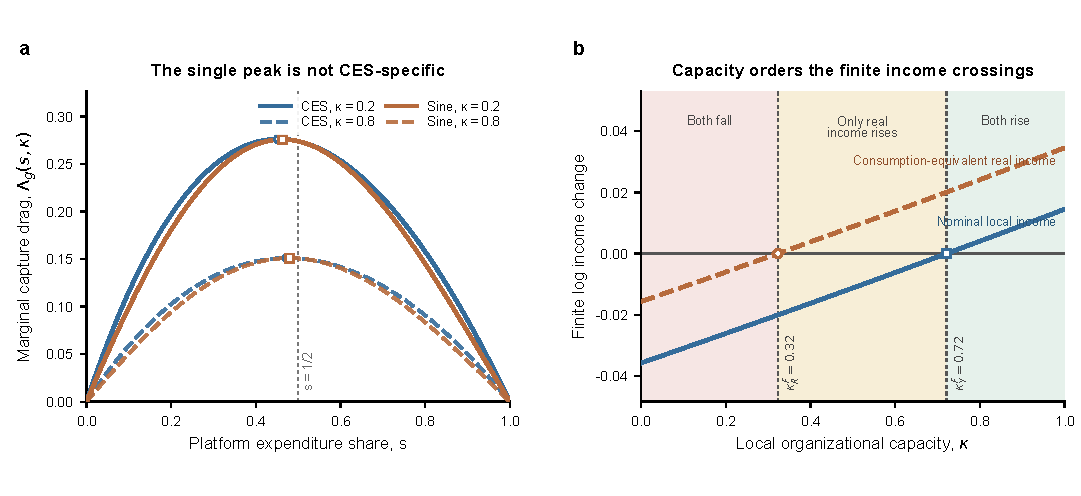
\includegraphics[width=\textwidth]{mechanism_figure.pdf}
\caption{当前论文的机制图。左图比较 CES 与 non-CES share-speed 的 capture drag；右图
展示有限变化下两个能力阈值。图形是机制说明，不是参数校准。}
\end{figure}

\subsection{Panel a：单峰不是 CES 特有结论}

横轴是平台支出份额 \(s\)，纵轴是边际 capture drag。蓝色 CES 曲线和棕色 sine 曲线都
先升后降，说明单峰来自 share-speed 的形状限制，而不是某个 CES 闭式解。虚线表示较高
能力 \(\kappa=.8\)：平台与本地代理渠道的留值差更小，所以峰值下降并向右移动。

\subsection{Panel b：能力排列有限收入结果}

横轴是组织能力 \(\kappa\)，纵轴是从 \(z_0\) 到 \(z_1\) 的有限 log-income change。
橙色虚线先在 \(\kappa_R^F=.32\) 过零，因为实际收入获得价格收益；蓝色实线随后在
\(\kappa_Y^F=.72\) 过零。由此形成“都下降—只有实际收入上升—都上升”三个区域。

\section{CES 只是一个可计算特例}

一般模型包含下面的 CES 聚合器：
\[
M=\left[(1-a)^{1/\eta}M_A^{(\eta-1)/\eta}
+a^{1/\eta}M_P^{(\eta-1)/\eta}\right]^{\eta/(\eta-1)},
\qquad a\in(0,1),\ \eta>1.
\]
支出最小化得到
\begin{align*}
P_M(z)&=\left[(1-a)p_A^{1-\eta}
+ap_P(z)^{1-\eta}\right]^{1/(1-\eta)},\\
s(z)&=\frac{ap_P(z)^{1-\eta}}
{(1-a)p_A^{1-\eta}+ap_P(z)^{1-\eta}},\\
s'(z)&=(\eta-1)s(1-s).
\end{align*}
因此 CES 对应
\[
g(s)=(\eta-1)s(1-s),
\]
它满足 M2 的形状条件。参数 \(a\) 是 CES 权重，不是平台市场份额；\(\eta\) 是渠道间
替代弹性。一般 M1--M3 不需要 \(a\) 或 \(\eta\)，它们只在需要显式计算 \(P_M\)、\(s\)
和图形时出现。

\begin{commonerror}
从 CES 得到的具体闭式峰值或二阶导数不能自动升级为一般需求系统结论。当前论文的一般 M2
依靠 \(g\) 的端点、内部正值和严格凹性证明唯一峰值；CES 是满足这些条件的一个例子。
\end{commonerror}

\section{模型证明了什么，没有证明什么}

\begin{center}
\small
\begin{tabularx}{\textwidth}{X X}
\toprule
模型证明的内容 & 模型没有证明的内容 \\
\midrule
一般 homothetic 两渠道需求下的价格和份额恒等式 & 平台如何战略定价或选择佣金 \\
给定 endpoint crossing 时的两个有限能力阈值 & 所有参数下都存在两个内部阈值 \\
严格凹 share-speed 下 capture drag 唯一单峰 & 峰值是社会最优平台份额 \\
\(G=0\) 下对数收入的 increasing differences & 最优能力投资或具体补贴额度 \\
消费等价实际收入 \(R\) 的变化 & 包含劳动、能力建设、住房和迁移成本的完整福利 \\
短期 small-open-region 收入闭合 & 多地区工资、人口和企业区位的一般均衡反馈 \\
\bottomrule
\end{tabularx}
\end{center}

还要注意 \(G>0\) 的边界。此时
\[
Y=\frac{B+\omega G}{D},
\]
定义
\[
\mathcal N=\frac{B_1+\omega_1G}{B_0+\omega_0G},
\]
正确的有限比率是
\[
\frac{Y_1}{Y_0}=\frac{\mathcal N}{\calD},
\qquad
\frac{R_1}{R_0}=\frac{\mathcal N}{\calD\calP^\alpha}.
\]
因为 \(\mathcal N\) 本身也随 \(\omega\) 和 \(\kappa\) 变化，M1 的简洁闭式能力阈值专门
在 \(G=0\) 下陈述，不能把 \(\calB/\calD\) 或本讲义的两个阈值公式直接套到 \(G>0\)。

\section{两次 90 分钟的建议讲授顺序}

\subsection*{第一讲：需求、留值与收入循环}
\begin{enumerate}
  \item 15 分钟：用 100 元订单区分交易额与本地收入；
  \item 20 分钟：Cobb--Douglas 外层问题、\(Y\) 与 \(R\)；
  \item 20 分钟：一般单位支出函数、Shephard identity 与平台份额；
  \item 15 分钟：\(\rho_P\)、\(\Delta\)、\(\omega\) 与组织能力；
  \item 20 分钟：收入固定点、几何级数与 \(m_B\)、\(\MG\)。
\end{enumerate}

\subsection*{第二讲：M1--M3 与机制图}
\begin{enumerate}
  \item 30 分钟：M1 有限变化、endpoint crossing 与三个能力区域；
  \item 25 分钟：M2 share-speed、单峰直觉和 CES／sine 对照；
  \item 15 分钟：M3 increasing differences 及其边界；
  \item 10 分钟：两面板机制图；
  \item 10 分钟：练习讨论与常见误解。
\end{enumerate}

\section{课堂练习}

\subsection{基础题}
\begin{enumerate}
  \item 将下列对象分别归入“支出”“进入模型前已形成的本地收入”“均衡结果”三类：游客
  在本地消费、外销增加值、居民平台交易额、\(B\)、\(G\)、\(Y\)。

  \item 已知 \(\alpha=.4\)、\(\beta=.2\)、\(Y=1000\)、\(P_M=.8\)，求三类商品的支出，
  并写出 \(R\) 相对于 \(Y\) 的表达式。

  \item 已知 \(\alpha=.35\)、\(\beta=.25\)、\(\omega=.7\)，计算 \(D\)、\(m_B\) 和
  \(\MG\)，并解释为什么 \(m_B>\MG\)。

  \item 若 \(s=.4\)、\(\rho_A=.75\)、\(\rho_P=.45\)，求 \(\Delta\) 和 \(\omega\)。
  当平台份额上升时，平均留值率向哪个方向变化？
\end{enumerate}

\subsection{理解与应用题}
\begin{enumerate}[resume]
  \item 在 M1 数值例子中，地区能力为 \(\kappa=.5\)。判断 \(Y\) 和 \(R\) 的有限变化，
  并说明为什么两者符号不同。

  \item 设 \(\calD(0)=1.08\)、\(\calD(1)=1.01\)、\(q_R^F=1.10\)、
  \(q_Y^F=1.05\)。是否存在两个内部阈值？若不存在，指出失败的条件。

  \item 证明在 \(0<\calP<1\) 时 \(q_R^F>q_Y^F\)，并用 \(\calD(\kappa)\) 严格递减
  解释为什么 \(\kappa_R^F<\kappa_Y^F\)。

  \item 对称 share-speed 满足 \(g'(1/2)=0\)。利用
  \(F(1/2,b)=-bg(1/2)<0\) 解释为什么峰值严格小于 1/2。

  \item 用一句不涉及“最优政策”的话准确解释 M3。再列出 M3 的三个限定：关于 \(G\)、
  收入变换和能力性质各一个。

  \item 分别讨论 \(\Delta>0\)、\(\Delta=0\)、\(\Delta<0\) 时
  \(\Lambda_g\) 的经济解释。哪些情况下 M2 的 drag-peak 命题适用？
\end{enumerate}

\clearpage
\section{参考答案}

\begin{enumerate}
  \item 游客消费、居民平台交易额和 \(G\) 是支出；外销增加值和 \(B\) 是进入模型前已经
  形成的本地收入；\(Y\) 是所有传播轮次完成后的均衡名义本地收入。

  \item 零售、本地非贸易品和外部商品支出分别为 400、200 和 400。实际收入为
  \[
  R=K\frac{1000}{(.8)^{.4}},
  \quad K=(.4)^{.4}(.2)^{.2}(.4)^{.4}.
  \]

  \item
  \[
  D=1-.25-.35(.7)=.505,
  \quad m_B=1/.505\approx1.9802,
  \quad \MG=.7/.505\approx1.3861.
  \]
  \(B\) 已是本地收入，而 \(G\) 的第一轮只有比例 \(\omega\) 成为本地收入，因此
  \(m_B>\MG\)。

  \item \(\Delta=.75-.45=.30\)，
  \(\omega=.6(.75)+.4(.45)=.63\)。因为 \(\Delta>0\)，平台份额上升使
  \(\omega\) 下降。

  \item \(\kappa=.5\) 位于 .323162 和 .721929 之间，所以
  \(Y_1/Y_0=.988803<1\)，\(R_1/R_0=1.008837>1\)。价格指数下降带来的购买力收益
  足以抵消实际收入中的 capture loss，但还不足以让名义收入转正。

  \item 不存在两个内部阈值，因为 \(q_R^F=1.10>\calD(0)=1.08\)，实际收入目标没有落在
  \((\calD(1),\calD(0))\) 内。endpoint-crossing 条件失败。

  \item 因 \(\calP^\alpha<1\)，
  \(q_R^F=\calB/\calP^\alpha>\calB=q_Y^F\)。严格递减函数的反函数也递减，所以较大的
  目标 \(q_R^F\) 对应较小的能力阈值。

  \item \(F\) 随 \(s\) 严格下降。它在 0 处为正，而在 1/2 已经为负，所以唯一零点必位于
  \((0,1/2)\)。该零点就是 \(\Lambda_g\) 的唯一峰值。

  \item 准确表述示例：“在 \(G=0\) 的基准下，整合越深，提高一单位外生组织能力带来的
  对数名义收入和对数实际收入增益越大。”三个限定是：\(G=0\)；结论针对 \(\ln Y\)、
  \(\ln R\)；\(\kappa\) 是外生 retention shifter，模型没有能力成本或最优选择。

  \item \(\Delta>0\) 时平台留值较低，\(\Lambda_g>0\) 是 capture drag，M2 适用；
  \(\Delta=0\) 时 \(\Lambda_g\equiv0\)，没有唯一峰值；\(\Delta<0\) 时
  \(\Lambda_g<0\)，平台扩张提高平均留值，不能解释为拖累。因此 M2 明确要求
  \(\Delta(\kappa)>0\)。
\end{enumerate}

\section{五个方程回顾整套机制}

本科生掌握以下五个方程，就能复原模型主线：
\begin{align*}
s&=\frac{\partial\ln P_M}{\partial\ln p_P},
&\frac{d\ln P_M}{dz}&=-s,\\
\omega&=\rho_A-s\Delta(\kappa),
&Y&=\frac{B+\omega G}{1-\beta-\alpha\omega},\\
\frac{Y_1}{Y_0}&=\frac{\calB}{\calD(\kappa)},
&\frac{R_1}{R_0}&=\frac{\calB}{\calD(\kappa)\calP^\alpha},\\
s'(z)&=g(s),
&\Lambda_g&=\frac{\alpha\Delta(\kappa)g(s)}
{d_A+\alpha\Delta(\kappa)s},\\
\frac{\partial^2\ln Y}{\partial z\,\partial\kappa}
&=\frac{\partial^2\ln R}{\partial z\,\partial\kappa}
=\frac{\alpha\delta_\rho d_A s'(z)}{D^2}>0\quad(G=0).
\end{align*}

第一行连接价格与需求份额；第二行连接渠道重组与地方收入循环；第三行给出 M1 的有限变化；
第四行给出 M2 的一般边际拖累；第五行给出 M3 的互补性。中心结论不是平台化必然“好”或
“坏”，而是同样的整合冲击会因地方价值捕获结构和组织能力不同，产生不同的名义收入与
消费购买力结果。

\bigskip
\noindent\textbf{配套文件：}
\begin{itemize}[leftmargin=2em,itemsep=0.1em,topsep=0.2em]
  \item 投稿主稿：\texttt{paper/main.tex}；
  \item 证明：\texttt{paper/appendix.tex}；
  \item CES 与边界细节：\texttt{paper/supplement.tex}。
\end{itemize}
本讲义是独立教学材料，不改变这些正式文件，也不覆盖旧讲义。

\end{document}
